%
% Poorman's Hangul Jamo Input Method
% pmhanguljamo.sty 사용설명서
%
% (C) 2020 Nova de Hi.
% 		part of pmhanguljamo package.
%
\documentclass[a4paper]{oblivoir}

\hypersetup{colorlinks}

\usepackage{fapapersize}
\usefapapersize{*,*,1in,*,1in,*}

\usepackage{kotex-logo}
\usepackage{amssymb}
\usepackage{pmhanguljamo}
\usepackage{boxedminipage}

\ifXeTeX
\def\fontfeatureoption{Script=Hangul}
\else\ifLuaTeX
\def\fontfeatureoption{Script=Hangul,RawFeature={mode=harf}}
\fi\fi

%%% [Script=Hangul] is needed to typeset YETHANGUL
\setmainfont{Noto Serif}
\setsansfont{Noto Sans}
\setmonofont{Noto Sans Mono}
\setsansfont{Noto Sans CJK KR}[\fontfeatureoption]
\setkomainfont(Noto Serif CJK KR)(* Bold)(Noto Sans CJK KR Light)[\fontfeatureoption]
\setkosansfont(Noto Sans CJK KR)(* Bold)[\fontfeatureoption]
\setkomonofont(Noto Sans Mono CJK KR)

\usepackage{tcolorbox}
\tcbuselibrary{listings,breakable}
\tcbset{listing engine=listings,colframe=gray,colback=white,size=normal}
\NewDocumentEnvironment {exampleside} {}
  { \tcblisting{listing side text,righthand width=.38\textwidth} }
  { \endtcblisting }

\newcommand\pkg[1]{%
	\textsf{#1}\index{#1}\index{패키지!#1}%
}

\newcommand\env[1]{%
	\textit{<#1>}\index{환경!#1}\index{#1}%
}

\let\cmda\cmd

%\makeindex
\parindent=0pt

\begin{document}

\title{Poorman's Hangul Jamo Input Method \\ \large pmhanguljamo.sty}
\author{Nova de Hi}
%\date{2020/07/17\quad v0.1}
%\date{2020/07/18\quad v0.1.1}
%\date{2020/07/19\quad v0.2.0}
%\date{2020/01/20\quad v0.2.1}
%\date{2020/01/28\quad v0.3}
%\date{2020/01/30\quad v0.3.1}
%\date{2020/02/05\quad v0.3.2}
%\date{2020/03/09\quad v0.3.3}
%\date{2020/03/15\quad v0.3.4}
%\date{2020/03/10\quad v0.3.5}
\date{2021/09/20\quad v0.3.6}

\maketitle

\begin{exampleside}
\begin{jamotext}
g@/r@/mi p@/r@/ni sai de/ug h@i/o/,\\
moy/hi pe/re/h@/ni gos/ bi/ci bvr bvd/n@n d@s/do/da/.\\
ors bo/mi bon/d@in sdo di/na/ga/n@/ni \\
e/nv na/ri i do/ra/gar h@i/o/.
\end{jamotext}
\end{exampleside}

\tableofcontents*

\section{목적}

\pkg{pmhanguljamo.sty}는 ``Poorman's Hangul Jamo Input Method''에서 따온 이름이다.
알파벳과 몇 개의 기호문자만으로 한글 자모 (첫가끝) 입력을 대신할 수 있게 만든 것이다.
자모 조합 한글을 잘 처리할 수 있는 폰트의 도움을 받아 (\ref{sec:font}절을 보라) `모든' 한글 수백만자를 표현할 수 있다.
한글 패키지 \koTeX 과 함께 쓸 수 있고, 단독으로 사용해도 한글 표현이 가능하다.
외국어를 본문으로 하고 한두 글자의 한글만을 표현할 필요가 있을 때, 별도의 입력기가 없는
상황에서 `옛한글'을 포함하는 문자와 문장을 출력하여야 할 때 쓸 수 있다.

\hologo{XeLaTeX}, \hologo{LuaLaTeX}에서 사용할 수 있고 
\hologo{pdfLaTeX}은 지원하지 않는다.

\section{사용법}

\subsection{패키지 사용 선언}

\begin{boxedverbatim}
\usepackage[<option>]{pmhanguljamo}
\end{boxedverbatim}

preamble에 위의 문장을 둔다. 옵션으로 \verb|rrk| 또는 \verb|RRK| 하나를 쓸 수 있는데
이 옵션은 ``표준 전자법''으로 현대 한글을 입력하는 방식으로 바뀐다. 이에 대해서는 
\ref{sec:rrk}절을 보라.
옵션을 주지 않으면 \ref{sec:pmrule}절에서 설명하는 pm 입력 방식을 따른다.

\subsection{명령과 환경}

\subsubsection{주의사항}

이 패키지의 목적은 한글 자모를 입력하여 한글이 표현되게 하는 것이다.
그러므로 한글이 입력되고 있는 범위(이하 “인자 범위”라고 부른다) 안에서는
원칙적으로 다른 어떤 매크로도 올 수 없다. 글자가 먼저 만들어져야 거기에 대해서
어떤 명령을 수행할 수 있기 때문이다. 예를 들어
\begin{verbatim}
    \textbf{\jamoword{<args>}}
\end{verbatim}
이것은 원하는 결과를 내지만
\begin{verbatim}
    \jamoword{\textbf{<args>}}
\end{verbatim}
이렇게 하면 오류가 발생한다.

\subsubsection{\texttt{\bs jamoword} 명령}

\begin{boxedverbatim}
\jamoword{<several words>}
\end{boxedverbatim}

한글 자모를 알파벳으로 입력하여 출력한다. 
하나 또는 둘 이상의 단어가 올 수 있다. (단 하나의 단어만을 처리하는 \cmda{\jamotextcmd}라는 명령이
있기는 하나 내부적으로 사용되는 것이다.) 
\verb|\par|를 포함하는 문단은 올 수 없다.

\medskip

\begin{exampleside}
\jamoword{na/ras;mar:ss@/mi; dyuq/guig;ei dar/a;} 
\end{exampleside}

\subsubsection{\env{jamotext} 환경}

\begin{boxedverbatim}
\begin{jamotext} 
<text>
\end{jamotext}
\end{boxedverbatim}

\env{jamotext} 환경은 여러 문단을 포함하는 긴 문장을 식자할 수 있다.
단 이 환경 안에 오는 모든 텍스트는 문장부호와 몇 가지 예외적인 것 이외에
인자를 취하는 매크로를 포함하지 않고 순수한 한글로만 되어 있어야 한다.

\medskip
\begin{exampleside}
\begin{jamotext}
na/ras;mar:ss@/mi; dyuq/guyg;ey; dar/a;

mun/jj@x;oa;ro; se/rv s@/m@s/di; a/ni;h@r/ss@i;
\end{jamotext}
\end{exampleside}

\subsubsection{\texttt{\bs jmcc} 명령}

\begin{boxedverbatim}
\jmcc{<single jamo>}
\end{boxedverbatim}

음절이 아니라 한 개의 자모만을 표시할 목적으로 \href{https://en.wikipedia.org/wiki/Hangul_Compatibility_Jamo}{한글 호환 자모}를 식자하려 할 때 사용하는 명령이다.
호환 자모를 \cmda{\jamoword} 명령의 인자 안에서 쓰는 방법은 \ref{sec:compjamo}절을 보라. 이 명령은 본문
중에서 독립적으로 쓰기 위해 마련되었다.
인자로 단 하나의 자모만이 와야 한다. 설령 \texttt{RRK} 옵션을 부여하여 RRK 입력 방법을 쓰는 때라도
이 명령의 인자는 이 패키지의 고유한 전자 규칙을 따른다. 쌍아래아는 유니코드 호환 자모에는 정의되어 있지
않으나 편의를 위하여 조판할 수 있도록 해두었다.

\medskip
\begin{exampleside}
\jmcc{BSG} \jmcc{@} \jmcc{UEY} \jmcc{@@}
\end{exampleside}

\section{轉字 규칙} \label{sec:pmrule}

이 패키지는 아래에서 설명하는 바 독특한 입력 문자 대응 규칙을 정의하여 쓴다. 이 방법을
편의상 ‘pm 전자 규칙’이라고 부르기로 한다. 이 방법은 \ref{sec:rrk}절에서 설명할 RRK 입력 규칙과
다르고 둘 중 하나를 선택하여 써야 한다. 소실된 한글 옛문자를 
완벽하게 식자하려면 pm 입력 방식으로만 가능하다.

\subsection{성조표지와 음절}

입력에는 로마자 알파벳과 \verb|@| 부호, 그리고 세 개의 성조표지(방점) 기호 \verb|/|, \verb|;|, \verb|:|를 사용하며, 중성 필러를 표현하기 위하여 \verb|*| 부호를 쓴다.

\emph{성조표지가 와야 음절이 완성된 것으로 본다}. 모든 한글 음절은 반드시 성조표지로 끝난다.
평성이 아닌 성조표지는 (적절한 폰트에서) 한글 음절의 왼편에 찍힌다.

\begin{table}[htpb]
\centering
\caption{성조 표지} \label{tab:tonemarker}
\begin{tabular}{l|l|l}
\hline
\texttt{/} & 평성 & 점 없음 \\ \hline
\texttt{;} & 거성 & 점 하나 (\jamoword{m@s;no/p@n; so/ri;}) \\ \hline
\texttt{:} & 상성 & 점 둘 \\ \hline
\end{tabular}
\end{table}

성조 표기를 하지 않는 경우에도 음절의 완성을 나타내는 \verb|/|를 두어야 한다. 
다만 이 경우에 입력 편의를 위한 예외로서 
그 뒤에 스페이스가 와서 단어 입력이 종료되는 위치(또는 입력 문자열의 마지막)에서는 \verb|/|를 생략할 수 있다. 다음 예를 보아라.

\medskip
\begin{exampleside}
\jamoword{naix:jyuq/ G/ so/ri;n@n;}\\
\jamoword{naix:jyuq G so/ri;n@n;}
\end{exampleside}

스페이스 앞에서 \verb|/|를 생략할 수 있음과 관련하여 스페이스가 아니라면 생략할 수 없음에 주의하라. 예컨대 마침표와 같은 문장부호가 올 때는 그 문장부호 앞에서 \verb|/|를 생략할 수 없다.

\medskip
\begin{exampleside}
\jamoword{jas ans bo/m@i pvr/oa na/mo/sbun gi/peys/do/da/.}
\end{exampleside}

\subsection{알파벳 대응 문자}

알파벳 소문자를 이용하여 한글 자모 영역의 문자를 입력한다. 자음과 모음의 대응 규칙은 다음과 같다.

\subsubsection{자음}

\begin{table}[h]
\centering
\caption{알파벳-자모 대응 규칙: 자음}\label{tab:cons}
\ttfamily
\begin{tabular}{ll|ll|ll|ll|ll}
\hline
ㄱ & g & ㄴ & n & ㄷ & d & ㄹ & r & ㅁ & m \\
ㅂ & b & ㅅ & s & ㅇ & \textbf{x} & ㅈ & j & ㅊ & c \\
ㅋ & k & ㅌ & t & ㅍ & p & ㅎ & h & & \\ \hline
\char"3181 & \textbf{q} & \char"317F & \textbf{z} &
\char"3186 & \textbf{f} & & & & \\
\hline 
\end{tabular}
\end{table}

\begin{enumerate}[1)] \firmlist
\item \texttt{g}, \texttt{n}, \texttt{d}, \texttt{r}, \texttt{m}, \texttt{b}, \texttt{s}, \texttt{j}, \texttt{c}, \texttt{k}, \texttt{t}, \texttt{p}, \texttt{h}는 연상이 가능할 것이므로 따로 설명하지 않는다. \jmcc{R}에 대하여
\verb|r|만을 사용하고 \verb|l|을 쓰지 않는다.
\item `\jmcc{X}'(이응)에 대하여 \verb|x|를 채택하였다. 원래 이것은 오래 전 \pkg{frktex}이라는 패키지에서 
첫소리 이응에 대하여 \verb|x|를 썼던 적이 있으므로 그 유래가 아주 없다고 할 수는 없겠다. 다만 이 패키지는 
종성 이응 받침도 \verb|x|를 쓴다. 
\item `\jmcc{Q}'(옛이응)을 \verb|q|로 한 것은 역시 \pkg{frktex}에서 온 것인데 ``꼭지 달린 이응''이라는 글자 모양이 \verb|q|를 연상시킨다''는 이유였다고 한다. 그럴 법도 하다.
\item `\jmcc{Z}'(반시옷)을 \verb|z|로 한 것은 납득할 수 있다고 본다. z가 s의 유성음에 대응하기 때문에.
\item 가장 곤란했던 것은 \jmcc{F}(여린히읗)이었다. 사용되지 않은 자판 가운데서 선택할 수밖에 없는데 \texttt{l}, \texttt{v}, \texttt{w}, \texttt{f} 정도가 선택 가능한 범위였다. 알파벳이 아닌 부호문자 중에서 선택하는 것도 생각해보았으나 역시 자판의 윗줄로 올라가는 것은 꺼려져서 \verb|f|로 선택하였다. 순전히 편의에 의한 대응이다.
\item `\jamotextcmd{sl@}'나 `\jamotextcmd{slr@}'와 같은 특별한 글자, `\jamotextcmd{jl*/cl*/jjl*/sl*/ss*}, \jamotextcmd{jlr*/clr*/jjlr*/slr*/sslr*}'의 초성 글자들, 즉 훈민정음 언해의 ``\jamoword{dyuq/guyg;so/ri;yeys; ni;sso/ri;}'' 표기에서 쓰이는 齒頭\cntrdot 正齒音을 구분하기 위한 글자들은 \texttt{s}, \texttt{j}, \texttt{c}에 \texttt{l}, \texttt{lr}을 붙여서 표기한다. \verb|l|이 왼쪽(치두음), \verb|lr|이 오른쪽(정치음)이 더 길어지는 글자가 된다.
\item `\jmcc{BX}', `\jmcc{BBX}', `\jmcc{MX}', `\jmcc{PX}'와 같은 ``\jamoword{ib/si/ur;ga/b@i;ya/bx@n; so/ri;}'' 표기는 \verb|x|를 이어써서 표기한다. 각각, \texttt{bx}, \texttt{bbx}, \texttt{mx}, \texttt{px}.
\item 겹자음\cntrdot 복자음은 이어쓴다. \texttt{gg} \jmcc{GG}, \texttt{bsg} \jmcc{BSG}, \texttt{bsd} \jmcc{BSD}, \texttt{rf} \jmcc{RF}.
\item `제로자음'인 초성 이응은 생략할 수 있다. 모음으로 시작하면 초성 이응을 식자해준다. \verb|\jamoword{an}| \jamoword{an}. 
\item 정말로 초성을 비우기를 원한다면(즉 초성 필러를 쓰려 한다면) \verb|w|를 그 위치에 쓸 수 있다. 이것은 종성에는 적용되지 않는다. \verb|\jamoword{wan}| \jamoword{wan}.
\end{enumerate}

\subsubsection{모음}

\begin{table}[h]
\centering
\caption{알파벳-자모 대응 규칙: 모음} \label{tab:vow}
\ttfamily
\begin{tabular}{ll|ll|ll|ll|ll}
\hline
ㅏ & a & ㅓ & e & ㅗ & o & ㅜ & u & ㅡ & \textbf{v} \\
ㅣ & i & \jmcc{@} & \textbf{@}  & & & & & & \\ \hline
ㅑ & ya & ㅕ & ye & ㅛ & yo & ㅠ & yu & \kern-.3em\jmcc{@}\kern-.6em\jmcc{@} & @@ \\ \hline
ㅐ & ay & ㅔ & ey & ㅚ & oy & ㅟ & uy & ㅢ & vy \\ 
ㅒ & yay & ㅖ & yey & \jmcc{YOI} & yoi & \jmcc{YUI} & yui & \jmcc{@I} & @i \\ \hline
ㅘ & oa & ㅙ & oay & ㅝ & ue & ㅞ & uey & & \\ \hline
\end{tabular}
\end{table}

\begin{enumerate}[1)]
\item 기본 모음 ㅏ, ㅓ, ㅗ, ㅜ, ㅡ, ㅣ, \jmcc{@}(\texttt{@})는 한 글자로만 표기한다. ㅑ, ㅕ, ㅛ, ㅠ는 \verb|y|를 앞에 붙인다.
\item `ㅡ'를 영문자의 자음에 해당하는 \verb|v|에 대응시킨 것은 이상하게 보일 수 있다. 그러나 윗 항을 충실하게 지키려다 보니 부득이했다. 실로 이 홀소리 글자의 로마자 표기는 혼란스럽다고 생각하고 있는데, 표준인 \texttt{eu}만이 아니라 \texttt{y}, \texttt{u} 등이 있었고, 다른 어떤 제안에서는 \verb|w|도 있었던 것으로 기억한다. 어차피 마땅한 방법이 없다면 이렇게 약속하고 쓰는 것이 한 방법이라 생각한다. \verb|v|자를 죽 늘리면 `ㅡ'가 되는 것처럼 보이는 연상에서 비롯되었는지 모른다.
\item \texttt{e}를 보통 `에'라고 읽기 때문에 `ㅓ'를 \verb|e|에 할당한 것이 익숙지 않을 수 있다. 이것은 Yale 표기법에 그 기원이 있다.
\item `ㅐ, ㅔ'는 단모음으로 간주되기 때문에 \texttt{ay}, \texttt{ey}라고 쓰도록 하였다. 비슷한 이유에서 \texttt{oy}, \texttt{uy}라고 되었다. 
그러나 이런 음성학적 지식이 표기에 반드시 필요하다면 그것도 불편하다. 그래서 `\texttt{ai}, \texttt{ei}, \texttt{oi}, \texttt{ui}'라고 입력하는 것도 허용하였다. `ㅢ'의 경우에도
\texttt{vy}와 \texttt{vi} 둘 다 가능하다.

\verb|\jamoword{sai/say}| \jamoword{sai/say}.\quad \verb|\jamoword{sei/sey}| \jamoword{sei/sey}. \\
\verb|\jamoword{soi/soy}| \jamoword{soi/soy}.\quad \verb|\jamoword{sui/suy}| \jamoword{sui/suy}. \\
\verb|\jamoword{gvi/gvy}| \jamoword{gvi/gvy}.

그러나 \jmcc{@I}는 단모음으로 인식될 가능성이 없다고 보아 \verb|@i|만을 취하였다. 

\verb|\jamoword{g@i}| \jamoword{g@i}.

\item `쌍아래아(\jmcc{@@})'는 현대의 제주어 표기에서 이따금 필요하다. 모양대로 \verb|@@|로 적으며 \verb|y@|를 취하지 않았다. 현대 국어에서 이 글자의 소리는 잊혀진 것이라서 소리로 연상할 수 없기 때문이다.\\
\verb|\jamoword{@@/nam/vn}| \jamoword{@@/nam/vn}.
\item 표준 로마자 표기법에서 \texttt{wa}, \texttt{wo}, \texttt{we}, \texttt{wi}로 표기할 때 나타나는 반자음 \verb|w|은 채택하지 않았다. `ㅘ, ㅝ, ㅟ'는 생긴 대로 \texttt{oa}, \texttt{ue}, \texttt{ui}로 적는다.
\item 이 패키지는 Unicode 4.0의 한글 자모 확장 A, B를 지원한다. 그러므로 한글 자모 영역([U+11XX])에는 없는 `\jamoword{wuye}'와 같은 모음을 표기할 수 있다. \verb|\jamoword{sa/guye}| \jamoword{sa/guye/}. 물론 폰트가 이를 지원해야 한다.
\item 중성 필러([U+1160])는 \verb|*| 부호로 적을 수 있다. \verb|\jamoword{h*n}| \jamoword{h*n}. 초성과 중성을 모두 filler로 채우는 경우에는 종성이 있어야 한다. \verb|\jamoword{w*f}| \jamoword{w*f}.
\end{enumerate}

\subsubsection{호환자모 음절} \label{sec:compjamo}

\cmda{\jamoword}나 \env{jamotext} 범위 안에서 호환 자모를 식자하려면 해당하는 자모를 대문자로, 하나의 음절로 입력한다.
별도로 \cmda{\jmcc}를 쓰지 않는다. 그러나 반드시 하나의 자모가 한 음절이어야 한다.

\begin{exampleside}
\jamoword{B/n@n; ib/si/ur;sso/ri;ni;} \\
\jamoword{孟m@ix/子j@/I g@r/@/sya/d@i}
\end{exampleside}

\medskip

호환 자모 아래아 `\jmcc{@}'를 \cmda{\jamoword} 인자 안에서 식자하려 할 때는 자모 아래아 `\jamoword{w@}'와
구별하기 위해 대문자 \texttt{W}로 표기해야 한다. \verb|W|, \verb|WW|, \verb|WI|만이 지원된다.

\begin{exampleside}
\jamoword{W/n@n; 呑t@n/D/字/jj@x; ga/on;d@is;so/ri; g@;t@;ni/ra;.}\\
\jamoword{WW/nvn jei/ju/e pyo/gi/ei i/yox/doin/da/.}
\end{exampleside}

\subsubsection{문장 부호, 한자와 음절 한글}

\cmda{\jamoword} 명령과 \env{jamotext} 환경 안에 오는 인자는 다음과 같은 문자에 대하여 예약이 되어 있다.
\begin{itemize}\firmlist
\item 알파벳 문자 --- 한글 자모 문자에 대응한다.
\item \texttt{;}, \texttt{:}, \texttt{/} --- 이 세 개의 부호는 성조표지, 음절완성을 표시하기 위하여 예약되어 있다.
\item \texttt{|} --- 이 한 개의 부호문자는 내부적으로 사용하도록 예약되어 있다.
\end{itemize}
이를 제외한 문자는 입력한 대로 찍힌다. 즉 한글 완성형 음절 문자나 한자 및 숫자와 문장부호가 모두 그대로 출력된다. 예: \verb|\jamoword{``/u/ri/na/ra/"}| \jamoword{``/u/ri/na/ra/"}. 모든 문장 부호는 모두 음절 분리 부호에 의하여 분리되어 있어야 한다는 점에 주의하라.

콜론, 세미콜론, 슬래시는 각각 \cmda{\ColonMark}, \cmda{\SemiColonMark}, \cmda{\SlashMark} 명령을 사용할 수 있게 해두었다.

\medskip
\begin{exampleside}
\jamoword{15 세기 표기\ColonMark{} 國之語音, 우리나라의 말이 $\Rightarrow$ na/ras/mar/ss@/mi}
\end{exampleside}

매크로를 쓸 수 없는 것이 원칙이기는 하나,
protect된 단일 매크로는 그대로 출력된다. 그러나 인자를 취하는 매크로는 오류가 발생할 것이므로 
인자 범위 밖에 두도록 하라.

%RRK 입력 방식이 활성화되면 매크로 사용은 더욱 제한된다. \cmda{\ColonMark}와 같은 임시 명령도 동작하지 않는다.

\medskip

음절문자뿐 아니라 자모 한글의 입력도 그대로 출력된다. 어디선가 옛한글%
\footnote{1933년 이전 표기법의 한글을 가리킨다.
유니코드의 한글 음절 문자 영역에서 표현되지 않는 한글을 통칭하는 것이나
현대 한국어 중에서 제주어를 기록할 때도 쓰이고, 워드 프로세서 \jamoword{h@n/gvr}의
이름을 적을 때도 쓰이기 때문에 그리 `옛' 것은 아니다.
이 글에서는 관행을 따라 옛한글이라고 부르기로 한다.}
텍스트를 복사해와서 넣을 때 유용할지도.
다음 예에서 이 패키지의 입력 방식과 첫가끝 입력 방식이 혼용되어 있는 것을 볼 수 있다.

\medskip
\begin{exampleside}
\jamoword{(/du/si/en/hai dvx/go/)
ᄇᆞᄅᆞ미 ᄲᆞᄅᆞ며 하ᄂᆞᆯ히 놉고 나ᄇᆡ 됫ᄑᆞ라미 슬프니}
\end{exampleside}

\section{폰트}

\subsection{사용가능한 글꼴}\label{sec:font}

자모 조합 한글을 출력하려면 이를 해낼 수 있는 글꼴이 필요하다. 소위 `옛한글' 글꼴이라지만 PUA 옛한글
5000여자의 사용자 영역 글자만을 가지고 있는 글꼴로는 이 패키지에서 말하는 옛한글을 식자할 수 없다. 새바탕\cntrdot 새굴림과 같은 한양 옛한글
폰트, 전주완판본체, 제주폰트 등이 모두 옛한글에 사용할 수 없는 폰트에 해당한다.

자모 조합 한글을 구현할 수 있는 몇몇 글꼴을 테스트해보겠다. 

\begin{boxedverbatim}
sa:r@m/ma:da; h@i:xxye; su:bxi; ni/gye;
\end{boxedverbatim}

\newcommand\teststr{\jamoword{sa:r@m/ma:da; h@i:xxye; su:bxi; ni/gye;
}}

\newcommand\testfont[1]{%
	\begingroup
	\begin{adjustwidth}{2em}{2em}
	\adhochangulfont[\fontfeatureoption]{#1}\teststr
	\end{adjustwidth}
	\endgroup
}

함초롬 바탕 \testfont{HCR Batang LVT}

은 바탕 \testfont{UnBatang}

본명조 또는 Noto Serif CJK \testfont{Noto Serif CJK KR}

나눔명조옛한글 \testfont{NanumMyeongjo-YetHangul.ttf}

KoPubWorld 바탕 \testfont{KoPubWorldBatangMedium}

함초롬 돋움 \testfont{HCR Dotum LVT}

본고딕 또는 Noto Sans CJK \testfont{Noto Sans CJK KR}

나눔바른고딕옛한글 \testfont{NanumBarunGothic-YetHangul.ttf}

맑은 고딕 \testfont{Malgun Gothic}

KoPubWorld 돋움 \testfont{KoPubWorldDotumMedium}

\medskip

옛한글을 무리없이 표현하는 것은 현재 이 정도인 것 같다.
각 폰트는 특정한 문자에 대해서 약간의 차이를 보이기도 한다. 참고로 이 문서에서는
본문과 옛한글에 Noto Serif CJK KR을 사용하였다.

\hologo{LuaTeX}으로 컴파일하는 경우에는 위에 든 폰트들, 즉 \texttt{Script Hangul} 속성을 
가진 폰트만 사용 가능하다. \hologo{LuaTeX}과 이 패키지의 관계에 대해서 
\pageref{sec:luatex}페이지를 참고하라.

\ifXeTeX

\bigskip

한글 자모 영역의 글리프를 가지고 있는 글꼴이 있다. 성조표지를 잘 처리하지 못하는 경우가 있고 옛한글
글자꼴이 반듯하지 않지만 어쨌든 글자가 나오기는 할 것이다. 이것은 \texttt{Script Hangul} 속성을 갖고
있는 것은 아니며 단지 한글 자모 영역 글리프를 영리하게 배열한 것이다. 방점 없이 테스트해보겠다.

\medskip

\renewcommand\teststr{\jamoword{sa/r@m/ma/da h@i/xxye su/bxi ni/gye
}}

은 자모바탕 \testfont{UnJamoBatang}

은 돋움 \testfont{UnDotum}

\medskip
그러나 자모 영역 자면이 있다 하더라도 글리프가 잘 조성되어 있지 않은 글꼴에서는
다음과 같이 모아쓰기가 되지 않는 형태로 출력된다. 이런 글꼴은 옛한글에 사용할 수 없다.

\medskip
전주완판본 순L \testfont{TSTJJWanSunL}

\medskip

\textbf{현대 한글 음절문자}는 적어도 \hologo{XeLaTeX}에서는 모두 제대로 표현될 것이다.
자모 코드로부터 한글 음절을 (유니코드 표준을 따라) 구성하는 일을 폰트가 아니라 \hologo{XeTeX}이 하고 있음을 짐작할 수 있다.\footnote{이 패키지의 입력 방법으로 \hologo{XeLaTeX} 컴파일하여 만들어진 현대 한글 음절 영역 문자를 pdf로부터
복사하여 편집기에 붙여넣기하면 자모 코드가 아니라 음절 코드로 들어가는 것을 확인할 수 있다.}
현대 한글만을 표기하려 한다면 폰트의 제약이 줄어든다고 하겠다.

\begin{boxedverbatim}
o/dvx/vn ja/ey a jo/sen/vi dog/rib/gug/im/goa
\end{boxedverbatim}

\renewcommand\teststr{\jamoword{o/dvx/vn ja/ey a jo/sen/vi dog/rib/gug/im/goa}}

백묵 바탕 \testfont{batang.ttf}

Adobe 명조 \testfont{AdobeMyungjoStd-Medium.otf}

전주완판본 순L \testfont{TSTJJWanSunL}

제주한라산 \testfont{JejuHallasan.ttf}

\fi

\subsection{폰트의 지정}

특정 언어 패키지나 입력기의 제약 없이 한글 글꼴을 지정하는 것만으로
현대 한글과 옛한글을 모두 표현할 수 있다는 것이 \pkg{pmhanguljamo}의 장점이다.
다만 \koTeX\ 없이는 글자 사이의 행나눔이나 양끝맞추기 등 한글 문장 식자에 꼭 필요한 몇 가지 기능이 구현되지 
않을 것이므로 이런 점은 감안하여야 한다. 대체로 몇 자 정도의 한글을 넣어야 하는 때에 유용하리라 본다.

\koTeX\ 패키지와 함께 쓸 때와 그렇지 않을 때를 나누어서 간단히 사용법을 보이겠다.

\subsubsection{\koTeX\ 문서}
만약 \koTeX\ (\pkg{xetexko} 또는 \pkg{luatexko})과 함께 사용하는 경우라면 본문 한글 글꼴을 
다음과 같이 지정한다. 

\texttt{[Script=Hangul]} \emph{옵션을 반드시 주어야 한다}는 점을 기억하자.\footnote{이것은 
폰트가 가지고 있는 오픈타입 속성을 활성화하여 자모 한글을 제대로 출력하도록 지정하는 역할을 한다. 자모 한글을
처리하는 기능을 가지고 있지 않은 글꼴에서는 아무 역할도 하지 않고 컴파일 시 콘솔에 경고 메시지를 보일 것이다.}%
\textsuperscript{, }\footnote{\hologo{LuaTeX}에서는 약간의
추가 옵션이 더 필요할 수 있다. 이 문서의 이후 \texttt{[Script=Hangul]}을 주라고 하는 때에
모두 동일하다. \pageref{sec:luatex}페이지의 부록 B를 보라.\label{fn:fontoption}}

\begin{boxedverbatim}
\setmainhangulfont{Noto Serif CJK KR}[Script=Hangul]
\end{boxedverbatim}

본문과 폰트를 달리 쓰려 한다면 \cmda{\jamoword} 또는 \env{jamotext} 범위에 다음과 같이 임시로 한글 글꼴을 적용한다.

\begin{boxedverbatim}
\hangulfontspec[Script=Hangul]{HCR Batang LVT}
\end{boxedverbatim}

\cmda{\adhochangulfont} 명령은 이와 동일한 명령이다. 이 폰트의 적용 범위를 설정하거나 하는 것은 문서작성자에게 맡겨져 있다.

\subsubsection{\koTeX 이 아닐 때}

\koTeX\ 문서가 아닐 때는 \pkg{fontspec} 패키지를 이용한다. main font를 위의 글꼴 중의 하나로 하거나(이 때에도 \texttt{[Script=Hangul]} 옵션을 반드시 지정하여야 한다.),
\cmda{\newfontfamily}로 글꼴 명령을 만들어 쓰거나,
아니면 한글이 필요한 부분에만 \cmda{\fontspec}으로 글꼴을 지정해주는 것으로 될 것이다.
%\fref{fig:sample}\는 \pkg{article} 문서의 한 예이다.
다음은 \pkg{article} 문서의 한 예이다.\footnote{폰트에 부여하는
옵션에 관하여 각주~\ref{fn:fontoption}\을 볼 것.}

%\begin{figure}
%\centering
%\begin{boxedminipage}{\dimexpr\textwidth-2.5cm\relax}
\begin{boxedverbatim}
\documentclass{article}
\usepackage{fontspec}
\newfontfamily\hngljmfont{HCR Batang LVT}[Script=Hangul]
\usepackage{pmhanguljamo}
\newcommand*\jmhangul[1]{%
    \begingroup
    \hngljmfont\jamoword{#1}%
    \endgroup
}

\begin{document}
Say `Hello' in Korean, 
\jmhangul{an/nyex/ha/sey/yo}.
\end{document}
\end{boxedverbatim}
%\end{boxedminipage}
%\caption{article에서 pmhanguljamo을 쓰는 예}\label{fig:sample}
%\end{figure}

\bigskip

\pkg{polyglossia}와 함께 사용하는 것도 잘 된다.
%\footnote{\pkg{polyglossia}는 \XeLaTeX 에서만 사용 가능하다.}
다음은 이 경우의 한 설정 방법이다.
(이 보기에서는 한국어를 other language로 설정하고 있는데 만약 main language로 설정한다면
\env{korean} 환경 안이 아니라도 한글 폰트가 적용된다.)
\pkg{polyglossia}를 사용하여 \env{korean} 환경에서
쓰게 되면 한국어 조판에 필요한 상당한 지원이 이루어진다.

\begin{boxedverbatim}
\documentclass{article}
\usepackage{polyglossia}
\setmainlanguage{english}
\setotherlanguage{korean}
\newfontfamily\hangulfont{UnBatang}[Script=Hangul]
\usepackage{pmhanguljamo}

\begin{document}
\begin{korean}
\jamoword{han/gug/e/rvr han/gvr/ro}
\end{korean}
\end{document}
\end{boxedverbatim}

만약에 \env{korean} 환경이 시작되면 그 안에서는 (무조건) pmjamo 입력 모드가 되도록 하려면
다음 코드를 preamble에 두면 된다.

\begin{boxedverbatim}
\usepackage{etoolbox}
\apptocmd\korean{\begin{jamotext}}{}{}
\pretocmd\endkorean{\end{jamotext}}{}{}
\end{boxedverbatim}

이제 다음과 같이 간단히 입력할 수 있다.

\begin{verbatim}
\begin{korean}
na/ras/mar/ss@/mi 
\end{korean}
\end{verbatim}

그러나 위의 처방은 이 환경 안의 모든 로마자가 한글이라는 확신이 있을 때만 적용해야 할 것이다.
\env{korean} 환경 안에서 로마자를 입력해야 할 일이 있을지 모르기 때문이다. 

\subsection{훈민정음 어제 서문}

훈민정음 어제 서문을 입력한 예를 보여두겠다.

\begin{boxedverbatim}
\begin{jamotext}
世syeyx;宗joq/御ex;製jyeyx;訓hun;民min/正jyeq;音fvm/

na/ras;mar:ss@/mi; 中dyuq/國guig;ei; dar/a;
文mun/字jj@x;oa;ro; se/rv s@/m@s/di; a/ni;h@r/ss@i;
i;ren jyen/c@;ro; e/rin; 百b@ig;姓syeq;i; ni/rv/go;jye; horf; bai; 
i/sye;do; m@/c@m;nai: jey bdv;dvr; si/re; pye/di; 
mod:h@rf no;mi; ha/ni;ra;.

nai; i;r@r; 爲uix;h@;ya; e:yes/bi; ne/gye; 
sai;ro; sv;mvr; ye/dvrb; 字jj@x;r@r; m@iq/g@;no/ni;
sa:r@m/ma:da; h@i:xxye; su:bxi; ni/gye;
nar;ro; bsu;mey; 
便bbyen/安fan/kvi; h@/go;jye; h@rf sd@/r@/mi;ni/ra;.
\end{jamotext}
\end{boxedverbatim}

\begin{quote}
\begin{jamotext}
世syeyx;宗joq/御ex;製jyeyx;訓hun;民min/正jyeq;音fvm/

na/ras;mar:ss@/mi; 中dyuq/國guig;ei; dar/a;
文mun/字jj@x;oa;ro; se/rv s@/m@s/di; a/ni;h@r/ss@i;
i;ren jyen/c@;ro; e/rin; 百b@ig;姓syeq;i; ni/rv/go;jye; horf; bai; i/sye;do;
m@/c@m;nai: jey bdv;dvr; si/re; pye/di; mod:h@rf no;mi; ha/ni;ra;.

nai; i;r@r; 爲uix;h@;ya; e:yes/bi; ne/gye; 
sai;ro; sv;mvr; ye/dvrb; 字jj@x;r@r; m@iq/g@;no/ni;
sa:r@m/ma:da; h@i:xxye; su:bxi; ni/gye;
nar;ro; bsu;mey; 
便bbyen/安fan/kvi; h@/go;jye; h@rf sd@/r@/mi;ni/ra;.
\end{jamotext}
\end{quote}


\section{표준 로마자 표기법 전자법 입력}\label{sec:rrk}

\let\Ajamoword\jamoword
\let\Ajamotext\jamotext
\let\endAjamotext\endjamotext
\let\jamoword\relax
\let\jamotext\relax
\let\endjamotext\relax
\ExplSyntaxOn
%
% subroutines of pmhanguljamo.sty
%  v0.3.2 (2020/02/05)
%  v0.3.3 (2020/03/09)
%  v0.3.4 (2020/03/15)
%  v0.4   (2021/11/28)
%  v0.5   (2022/09/02)
%  v0.5.1 (2022/09/06)
%  v0.5.2 (2022/09/07)
%
\seq_new:N \l_textjm_seq

\NewDocumentEnvironment { jamotext } { +b }
{
	\seq_set_split:Nnn \l_textjm_seq {\par} { #1 }
	\seq_map_indexed_function:NN \l_textjm_seq \jamo_word_rrk:nn
}{}

\cs_new:Npn \jamo_word_rrk:nn #1 #2
{
%	\jamoword { #2 }
	\seq_set_split:Nnn \l_inparpar_seq { ~ } { #2 }
	
	\seq_map_indexed_inline:Nn \l_inparpar_seq
	{
		\regex_match:nnTF { ^\!\{ } { ##2 }
		{
			\tl_set:Nn \l_tmpa_tl { ##2 }
			\regex_match:nnTF { ^\!\{(.+?)\}$ } { ##2 }
			{
				\regex_replace_once:nnN { ^\!\{(.+?)\}$ } { \1 } \l_tmpa_tl
				\l_tmpa_tl 
			}
			{
				\tl_set_eq:NN \l_tmpb_tl \l_tmpa_tl
				\regex_replace_once:nnN { ^\!\{(.+?)\}(.*)$ } { \1 } \l_tmpa_tl
				\l_tmpa_tl 
				\regex_replace_once:nnN { ^\!\{(.+?)\}(.*)$ } { \2 } \l_tmpb_tl
				\exp_args:No \jamoword { \l_tmpb_tl }
			}	
		}
		{
			\jamoword{ ##2 }
		}
		
		\int_compare:nT { ##1 < \seq_count:N \l_inparpar_seq }
		{ \space }
	}

	\int_compare:nT { #1 < \seq_count:N \l_textjm_seq }
	{ \par }
}


\tl_new:N \l_tmpz_tl

\NewDocumentCommand \jamoword { m }
{
  \group_begin:
  \bool_if:NT \opt_usepmfont_bool
  { \pm_hangulfontspec [\opt_pmfontfeature_tl] {\opt_pmfont_tl } }
  
	\seq_set_split:Nnn \l_tmpa_seq { ~ } { #1 }
	\seq_map_indexed_inline:Nn \l_tmpa_seq
	{
		\tl_set:Nn \l_tmpz_tl { ##2 }
		\exp_args:No \str_if_in:nnT { \l_tmpz_tl } { - }
		{ 
			\regex_replace_all:nnN { \- } { \/\- } \l_tmpz_tl
		}
		\exp_args:No \str_if_in:nnT { \l_tmpz_tl } { . }
		{ 
			\regex_replace_all:nnN { \. } { \/\. } \l_tmpz_tl
		}
		\exp_args:No \str_if_in:nnT { \l_tmpz_tl } { , }
		{ 
			\regex_replace_all:nnN { \, } { \/\, } \l_tmpz_tl
		}
		\exp_args:No \str_if_in:nnT { \l_tmpz_tl } { ! }
		{ 
			\regex_replace_all:nnN { \! } { \/\! } \l_tmpz_tl
		}
		\exp_args:No \str_if_in:nnT { \l_tmpz_tl } { ? }
		{ 
			\regex_replace_all:nnN { \? } { \/\? } \l_tmpz_tl
		}
		\exp_args:No \str_if_in:nnT { \l_tmpz_tl } { : }
		{ 
			\regex_replace_all:nnN { \: } { \/\: } \l_tmpz_tl
		}
		\exp_args:No \str_if_in:nnT { \l_tmpz_tl } { ; }
		{ 
			\regex_replace_all:nnN { \; } { \/\; } \l_tmpz_tl
		}

		\exp_args:No \str_if_in:nnTF { \l_tmpz_tl } { / }
		{
			\exp_args:NNno \seq_set_split:Nnn \l_tmpb_seq { / } { \l_tmpz_tl }
			\seq_map_function:NN \l_tmpb_seq \rrk_fn_outer:n
		}
		{
			\exp_args:No \rrk_a_word:n { \l_tmpz_tl }
		}
		\int_compare:nT { \seq_count:N \l_tmpa_seq > ##1 }
		{
			\space
		}
	}
	\group_end:
}

\cs_new:Npn \rrk_fn_outer:n #1
{
	\rrk_a_word:n { #1 }
}

\cs_new_nopar:Npn \rrk_a_word:n #1
{
	\seq_gclear:N \g_outsyl_tl

	\regex_match:nnTF { [a-zA-Z0 ] } { #1 } 
	{
		\exp_args:NNnx \seq_set_split:Nnn \g_tmpa_seq {} { \str_lowercase:f { #1 } }

		\int_step_inline:nn { 9 }
		{
			\seq_put_right:Nn \g_tmpa_seq { 0 }
		}

		\cho_fn:
		
		\seq_use:Nn \g_outsyl_tl { } 
	}
	{
		#1
	}
}

\cs_new:Npn \insert_out:n #1
{
	\seq_put_right:Nn \g_outsyl_tl { #1 }
}

\cs_new:Npn \prepare_three_tk:
{
	\seq_pop_left:NN \g_tmpa_seq \l_tmpa_tl
	\seq_pop_left:NN \g_tmpa_seq \l_tmpb_tl
	\seq_pop_left:NN \g_tmpa_seq \l_tmpc_tl
}

\cs_new:Npn \cho_fn:
{
	\prepare_three_tk:
	
	\str_case_e:nn { \l_tmpa_tl }
	{
% Zero 자음
		{ @ } { \insert_out:n { ᄋ } \restore_c: \restore_b: \restore_a: }
		{ a } { \insert_out:n { ᄋ } \restore_c: \restore_b: \restore_a: }
		{ e } { \insert_out:n { ᄋ } \restore_c: \restore_b: \restore_a: }
		{ i } { \insert_out:n { ᄋ } \restore_c: \restore_b: \restore_a: }
		{ o } { \insert_out:n { ᄋ } \restore_c: \restore_b: \restore_a: }
		{ u } { \insert_out:n { ᄋ } \restore_c: \restore_b: \restore_a: }
		{ w } { \insert_out:n { ᄋ } \restore_c: \restore_b: \restore_a: }
		{ y } { \insert_out:n { ᄋ } \restore_c: \restore_b: \restore_a: }
		
		{ g } { \insert_out:n { ᄀ } \restore_c: \restore_b: }
		{ n } { \insert_out:n { ᄂ } \restore_c: \restore_b: }
		{ d } { \insert_out:n { ᄃ } \restore_c: \restore_b: }
		{ l } { \insert_out:n { ᄅ } \restore_c: \restore_b: }
		{ r } { \insert_out:n { ᄅ } \restore_c: \restore_b: }
		{ m } { \insert_out:n { ᄆ } \restore_c: \restore_b: }
		{ b } { \insert_out:n { ᄇ } \restore_c: \restore_b: }
		{ c } { \insert_out:n { ᄎ } \restore_c: }
		{ h } { \insert_out:n { ᄒ } \restore_c: \restore_b: }
		{ x } { \insert_out:n { ᄋ } \restore_c: \restore_b: }

%		{ s } { \exp_args:No \str_if_eq:nnTF { \l_tmpb_tl } { s }
%				{ \insert_out:n { ᄊ } \restore_c: }
%				{ \insert_out:n { ᄉ  } \restore_c: \restore_b: } }
		{ s } {
			\str_case_e:nnF { \l_tmpb_tl } 
			{
				{ s } { \insert_out:n { ᄊ } \restore_c: }
				{ g } { \insert_out:n { ᄭ } \restore_c: }
				{ d } { \insert_out:n { ᄯ } \restore_c: }
				{ b } { \insert_out:n { ᄲ } \restore_c: }
				{ j } { \insert_out:n { ᄶ } \restore_c: }
			}
			{ \insert_out:n { ᄉ } \restore_c: \restore_b: }
		}
		{ j } { \exp_args:No \str_if_eq:nnTF { \l_tmpb_tl } { j }
				{ \insert_out:n { ᄍ } \restore_c: }
				{ \insert_out:n { ᄌ  } \restore_c: \restore_b: } }
		{ k } { \exp_args:No \str_if_eq:nnTF { \l_tmpb_tl } { k } 
				{ \insert_out:n { ᄁ } \restore_c: }
				{ \insert_out:n { ᄏ } \restore_c: \restore_b: } }
		{ t } { \exp_args:No \str_if_eq:nnTF { \l_tmpb_tl } { t }
				{ \insert_out:n { ᄄ } \restore_c: }
				{ \insert_out:n { ᄐ  } \restore_c: \restore_b: } }
		{ p } { \exp_args:No \str_if_eq:nnTF { \l_tmpb_tl } { p }
				{ \insert_out:n { ᄈ } \restore_c: }
				{ \insert_out:n { ᄑ } \restore_c: \restore_b: } }
		{ - } { \exp_args:Nno \str_if_in:nnTF { aeiouwy@ } { \l_tmpb_tl }
				{ \insert_out:n { ᄋ } \restore_c: \restore_b: }
				{ \insert_out:n { } \restore_c: \restore_b: \cho_fn: }
		}
	}
	\jung_fn:
}

\cs_new:Npn \jung_fn:
{
	\prepare_three_tk:

	\exp_args:No \str_if_eq:nnTF { \l_tmpa_tl } { 0 }
	{ \scan_stop: }
	{
		\str_case_e:nn { \l_tmpa_tl }
		{
			{ i } { \insert_out:n { ᅵ } \restore_c: \restore_b: }
			{ o } { \exp_args:No \str_if_eq:nnTF { \l_tmpb_tl } { e }
					{ \insert_out:n { ᅬ } \restore_c: }
					{ \insert_out:n { ᅩ  } \restore_c: \restore_b: } }
			{ u } { \exp_args:No \str_if_eq:nnTF { \l_tmpb_tl } { i }
					{ \insert_out:n { ᅴ } \restore_c: }
					{ \insert_out:n { ᅮ  } \restore_c: \restore_b: } }
			{ a } { \exp_args:No \str_if_eq:nnTF { \l_tmpb_tl } { e }
					{ \insert_out:n { ᅢ } \restore_c: }
					{ \insert_out:n { ᅡ  } \restore_c: \restore_b: } }
			{ e } { \str_case_e:nnF { \l_tmpb_tl }
					{
						{ o } { \insert_out:n { ᅥ } \restore_c: }
						{ u } { \insert_out:n { ᅳ } \restore_c: }
					}
					{ \insert_out:n { ᅦ } \restore_c: \restore_b: }
				  }
			{ @ } { \str_case_e:nnF { \l_tmpb_tl }
					{
						{ @ } { \insert_out:n { ᆢ } \restore_c: }
						{ i } { \insert_out:n { ᆡ } \restore_c: }
					}
					{ \insert_out:n { ᆞ } \restore_c: \restore_b: }
				  }
				  
			{ y } { \str_case_e:nn { \l_tmpb_tl }
					{
						{ o } { \insert_out:n { ᅭ } \restore_c: }
						{ u } { \insert_out:n { ᅲ } \restore_c: }
						{ a } { \exp_args:No \str_if_eq:nnTF { \l_tmpc_tl } { e }
								{ \insert_out:n { ᅤ } }
								{ \insert_out:n { ᅣ  } \restore_c: } }
						{ e } { \exp_args:No \str_if_eq:nnTF { \l_tmpc_tl } { o }
								{ \insert_out:n { ᅧ } }
								{ \insert_out:n { ᅨ  } \restore_c: } }
					}
				  }
			{ w } { \str_case_e:nn { \l_tmpb_tl }
					{
						{ o } { \insert_out:n { ᅯ } \restore_c: }
						{ i } { \insert_out:n { ᅱ } \restore_c: }
						{ e } { \insert_out:n { ᅰ } \restore_c: }
						{ a } { \exp_args:No \str_if_eq:nnTF { \l_tmpc_tl } { e }
								{ \insert_out:n { ᅫ } }
								{ \insert_out:n { ᅪ  } \restore_c: } }
					}
				  }
		}
	
		\jong_fn:
	}
}

\cs_new:Npn \prepare_five_tk:
{
	\seq_pop_left:NN \g_tmpa_seq \l_tmpa_tl
	\seq_pop_left:NN \g_tmpa_seq \l_tmpb_tl
	\seq_pop_left:NN \g_tmpa_seq \l_tmpc_tl
	\seq_pop_left:NN \g_tmpa_seq \l_tmpd_tl
	\seq_pop_left:NN \g_tmpa_seq \l_tmpe_tl
}

\cs_new:Npn \jong_fn:
{
	\prepare_five_tk:
	
	\exp_args:No \str_if_eq:nnTF { \l_tmpb_tl } { 0 }
	{
		\exp_args:Nx \insert_jong:n { \l_tmpa_tl }
	}
	{ 
		\exp_args:Nno \str_if_in:nnTF { aeiouwy@ } { \l_tmpb_tl }
		{ 
			\restore_e: \restore_d: \restore_c: \restore_b: \restore_a:
			\cho_fn:
		}
		{
			\exp_args:Nno \str_if_in:nnTF { aeiouwy@ } { \l_tmpc_tl }
			{ 
				\restore_e: \restore_d: \restore_c: \restore_b: \restore_a:
				\take_jong_two:
			}
			{
				\exp_args:Nno \str_if_in:nnTF { aeiouwy@ } { \l_tmpd_tl }
				{
					\restore_e: \restore_d: \restore_c: \restore_b: \restore_a:
					\take_jong_three:
				}
				{
					\exp_args:Nno \str_if_in:nnTF { aeiouwy@ } { \l_tmpe_tl }
					{ 
						\exp_args:Nx \insert_jong:n { \l_tmpa_tl \l_tmpb_tl }
%						\exp_args:Nx \insert_out:n { \l_tmpc_tl \l_tmpd_tl }
						\restore_e: \restore_d: \restore_c:
						\cho_fn:
					}
					{ 
						\restore_e: \restore_d: \restore_c: \restore_b: \restore_a:
						\take_jong_four:
					}
				}
			}
		}
	}
}

\cs_new:Npn \take_jong_four:
{
	\prepare_five_tk:
	\exp_args:No \str_if_eq:nnTF { \l_tmpa_tl } { 0 }
	{ \scan_stop: }
	{
		\exp_args:Nx \insert_jong:n { \tl_use:N \l_tmpa_tl \tl_use:N \l_tmpb_tl }
		\restore_e: \restore_d: \restore_c:
		\cho_fn:
	}
}

\cs_new:Npn \insert_jong:n #1
{
	\str_case:nn { #1 }
	{
		{ kk } { \insert_out:n { ᆩ } }
		{ gs } { \insert_out:n { ᆪ } }
		{ g }  { \insert_out:n { ᆨ } }
		{ nj } { \insert_out:n { ᆬ } }
		{ nh } { \insert_out:n { ᆭ } }
		{ n }  { \insert_out:n { ᆫ } }
		{ d }  { \insert_out:n { ᆮ } }
		{ lg } { \insert_out:n { ᆰ } }
		{ lm } { \insert_out:n { ᆱ } }
		{ lb } { \insert_out:n { ᆲ } }
		{ ls } { \insert_out:n { ᆳ } }
		{ lt } { \insert_out:n { ᆴ } }
		{ lp } { \insert_out:n { ᆵ } }
		{ lh } { \insert_out:n { ᆶ } }
		{ l }  { \insert_out:n { ᆯ } }
		{ m }  { \insert_out:n { ᆷ } }
		{ mg } { \insert_out:n { ᇚ } }	%% v0.4
		{ bs } { \insert_out:n { ᆹ } }
		{ b }  { \insert_out:n { ᆸ } }
		{ ss } { \insert_out:n { ᆻ } }
		{ s }  { \insert_out:n { ᆺ } }
		{ sg } { \insert_out:n { ᇧ } }  %% v0.4
		{ ng } { \insert_out:n { ᆼ } }
		{ j }  { \insert_out:n { ᆽ } }
		{ ch } { \insert_out:n { ᆾ } }
		{ k }  { \insert_out:n { ᆿ } }
		{ t }  { \insert_out:n { ᇀ } }
		{ p }  { \insert_out:n { ᇁ } }
		{ h }  { \insert_out:n { ᇂ } }
		{ / }  { \insert_out:n { 0 } }
	}
}

\cs_new:Npn \take_jong_three:
{
	\prepare_three_tk:
	\exp_args:No \str_if_eq:nnTF { \l_tmpa_tl } { 0 }
	{ \scan_stop: }
	{
%% XX-
	  \exp_args:No \str_if_eq:nnTF { \l_tmpc_tl } { - }
	  {
	    \exp_args:Nx \insert_jong:n { \l_tmpa_tl \l_tmpb_tl }
	    \restore_c:
	  }
	  {
	  	\exp_args:No \str_if_eq:nnTF { \l_tmpb_tl } { - }
	  	{
	    	\exp_args:Nx \insert_jong:n { \l_tmpa_tl }
	    	\restore_c: \restore_b:
	  	}
	  	{
			\check_jong_sub:
	  	}
	  }
	\cho_fn:
	}
}


\cs_new:Npn \check_jong_sub:
{
	\exp_args:Noo \str_if_eq:nnTF { \l_tmpb_tl } { \l_tmpc_tl }
	{
		\exp_args:Noo \str_if_eq:nnTF { \l_tmpa_tl } { \l_tmpb_tl } %%% sss
		{
			\exp_args:Nx \insert_jong:n { \l_tmpa_tl \l_tmpb_tl }  %% ss-s
			\restore_c:
		}
		{
			\bool_if:nTF {
				\exp_args:Noo \str_if_eq_p:nn { \l_tmpb_tl } { \l_tmpc_tl } %%% X-ss
				&&
				\exp_args:Noo \str_if_eq_p:nn { \l_tmpb_tl } { s }
			}
			{
				\exp_args:Nx \insert_jong:n { \l_tmpa_tl }
				\restore_c: \restore_b:
			}
			{
				\exp_args:Nno \str_if_in:nnTF { tpkj } { \l_tmpb_tl }
				{
					\exp_args:Nx \insert_jong:n { \l_tmpa_tl }
					\restore_c: \restore_b:
				}
				{
					\check_jong_sub_last:
				}
			}
		}
	}
	{
	  \str_if_eq:eeTF { \l_tmpa_tl } { k }
	  {
	  	\str_if_eq:eeTF { \l_tmpb_tl } { k } %% kk-g
		{
			\exp_args:Nx \insert_jong:n { \l_tmpa_tl \l_tmpb_tl }
			\restore_c:
		}
		{
			\exp_args:Nx \insert_jong:n { \l_tmpa_tl }
			\restore_c: \restore_b:
		}
	  }
	  {
		\exp_args:No \str_if_eq:nnTF { \l_tmpa_tl } { c }  %%% chX
		{
			\exp_args:Nx \insert_jong:n { \l_tmpa_tl \l_tmpb_tl }
			\restore_c:
		}
		{
			\exp_args:No \str_if_eq:nnTF { \l_tmpb_tl } { c } %%% Xch
			{
				\exp_args:Nx \insert_jong:n { \l_tmpa_tl }
				\restore_c: \restore_b:
			}
			{
				\check_jong_sub_last:
			}
		}
	  }
	}
}

\cs_new:Npn \check_jong_sub_last:
{
	\str_case_e:nnTF { \l_tmpa_tl }
	{
		{ n } { \str_case_e:nn { \l_tmpb_tl }
				{
					{ j } { }
					{ g } { }
					{ h } { }
				}
			  }
		{ g } { \str_case_e:nn { \l_tmpb_tl }
				{
					{ s } { }
				}
			  }
		{ l } { \str_case_e:nn { \l_tmpb_tl }
				{
					{ g } { }
					{ m } { }
					{ b } { }
					{ s } { }
					{ t } { }
					{ p } { }
					{ h } { }
				}
			  }
		{ b } { \str_case_e:nn { \l_tmpb_tl }
				{
					{ s } { }
				}
			  }
		{ s } { \str_case_e:nn { \l_tmpb_tl }
				{
					{ s } { }
				}
			  }
	}
	{
		\exp_args:Nx \insert_jong:n { \l_tmpa_tl \l_tmpb_tl }
		\restore_c:
	}
	{
		\exp_args:Nx \insert_jong:n { \l_tmpa_tl }
		\restore_c: \restore_b:
	}
}

\cs_new:Npn \take_jong_two:
{
	\prepare_three_tk:
	\exp_args:No \str_if_eq:nnTF { \l_tmpa_tl } { 0 }
	{ \scan_stop: }
	{
		\exp_args:Noo \str_if_eq:nnTF { \l_tmpa_tl } { \l_tmpb_tl }
		{ 
			\exp_args:Nno \str_if_in:nnTF { tpkj } { \l_tmpa_tl }
			{ \restore_c: \restore_b: \restore_a: }
			{
			  \exp_args:No \str_if_eq:nnTF { \l_tmpa_tl } { c }
				{ \restore_c: \restore_b: \restore_a: }
				{ \exp_args:Nx \insert_jong:n { \l_tmpa_tl }
	  	  			\restore_c: \restore_b: }
			}
		}
		{
			  \exp_args:No \str_if_eq:nnTF { \l_tmpa_tl } { c }
				{ \restore_c: \restore_b: \restore_a: }
				{ \exp_args:Nx \insert_jong:n { \l_tmpa_tl }
	  	  			\restore_c: \restore_b: }
		}
	}
	\cho_fn:
}

\cs_new:Npn \restore_c:
{
	\exp_args:NNx \seq_put_left:Nn \g_tmpa_seq { \tl_use:N \l_tmpc_tl }
}

\cs_new:Npn \restore_b:
{
	\exp_args:NNx \seq_put_left:Nn \g_tmpa_seq { \tl_use:N \l_tmpb_tl }
}

\cs_new:Npn \restore_a:
{
	\exp_args:NNx \seq_put_left:Nn \g_tmpa_seq { \tl_use:N \l_tmpa_tl }
}

\cs_new:Npn \restore_d:
{
	\exp_args:NNx \seq_put_left:Nn \g_tmpa_seq { \tl_use:N \l_tmpd_tl }
}

\cs_new:Npn \restore_e:
{
	\exp_args:NNx \seq_put_left:Nn \g_tmpa_seq { \tl_use:N \l_tmpe_tl }
}

\cs_new:Npn \restore_five:
{
	\restore_e: \restore_d: \restore_c: \restore_b: \restore_a:
}

\endinput

%% end of file pmhanguljamo-rrk.tex

\ExplSyntaxOff

패키지 옵션으로 \verb|[rrk]| 또는 \verb|[RRK]|가 주어지면 입력 규칙이 표준 로마자 표기법 전자법 방식으로
바뀐다. 전자법(transliteration method, 轉字法)이란 ``국어의 로마자 표기법'' (1998:2000) 제3장 제8항에서
\begin{quote}
학술 연구 논문 등 특수 분야에서 한글 복원을 전제로 표기할 경우에는 한글 표기를 대상으로 적는다. 이때 글자 대응은 제2장을 따르되 ‘ㄱ, ㄷ, ㅂ, ㄹ’은 ‘g, d, b, l’로만 적는다. 음가 없는 ‘ㅇ’은 붙임표(-)로 표기하되 어두에서는 생략하는 것을 원칙으로 한다. 기타 분절의 필요가 있을 때에도 붙임표(-)를 쓴다.
\end{quote}
라 규정한 방법을 말한다.\footnote{\url{https://www.korean.go.kr/front/page/pageView.do?page_id=P000150&mn_id=99}}
RRK는 이 문서의 영어 명칭인 \emph{Revised Romanization of Korean}의 첫 글자를 딴 것이다.
국어의 로마자 표기는 전음법이 원칙이고 전자법은 예외 규정이다. 그러나 한글의 입력 방법으로서 이를 쓰려 하는 한
전음법은 사용할 수 없다.

전자법 입력은 오직 현대어에만 적용된다. 따라서 옛한글은 이 방법으로 입력할 수 없다. (아래아 입력을 가능하게 한 것은
아래를 참조.)

\subsection{RRK 전자 규칙}

\begin{table}[h]
\centering
\begin{tabular}{ll|ll|ll|ll|ll|ll}
\hline
\multicolumn{12}{l}{자음}\\ \hline
ㄱ & g & ㄲ & kk & ㅋ & k & ㄷ & d & ㄸ & tt & ㅌ & t \\
ㅂ & b & ㅃ & pp & ㅍ & p & ㅈ & j & ㅉ & jj & ㅊ & ch \\
ㅅ & s & ㅆ & ss & ㅎ & h & & & & & & \\
ㄴ & n & ㅁ & m & ㅇ & ng & ㄹ & l & & & & \\ \hline
\end{tabular}
\end{table}

\begin{table}[h]
\centering
\begin{tabular}{ll|ll|ll|ll|ll|ll}
\hline
\multicolumn{12}{l}{모음} \\ \hline
ㅏ & a & ㅓ & eo & ㅗ & o &  ㅜ & u & ㅡ & eu & ㅣ & i\\ 
ㅐ & ae & ㅔ & e & ㅚ & oe & ㅟ & wi &  & & & \\ \hline
ㅑ & ya & ㅕ & yeo  & ㅛ & yo & ㅠ & yu & ㅒ & yae & ㅖ & ye \\
ㅘ & wa & ㅙ & wae & ㅝ & wo & ㅞ & we & ㅢ & ui & &  \\ \hline
 \end{tabular}
 \end{table}


\begin{enumerate}[(1)] \firmlist
\item 단어의 첫소리 `ㅇ'은 적지 않는다. 그밖의 초성 이응은 \verb|-|로 적는다. \\
\verb|\jamoword{annyeonghase-yo}|. \jamoword{annyeonghase-yo}.\\
\verb|\jamoword{na bogiga yeoggyeo-wo gasil ttae-eneun}| 
\jamoword{na bogiga yeoggyeo-wo gasil ttae-eneun}

\item 표준의 규정 대로 \verb|-|는 음절의 분철을 위해서 입력할 수 있다. 한편,
표준의 규정에는 없지만 음절 구분을 위한 \verb|/|를 사용할 수 있다. 음절 분리자가 쓰인
경우에는 초성 이응을 생략할 수 있다. \\
\verb|\jamoword{iss-eoss-seubnida}|. \jamoword{iss-eoss-seubnida}. \\
\verb|\jamoword{annyeonghase/yo}|. \jamoword{annyeonghase/yo}. \\
\verb|\jamoword{annyeonghase-yo}|. \jamoword{annyeonghase-yo}.

\item 모음과 모음 사이에 `ㅅ'이 세 개 오는 경우에는 쌍시옷 받침과 초성 시옷으로 분해한다. 만약 어떤 이유에선가 이 분철방법을
바꾸어야 한다면 \verb|-|나 음절 분리 부호를 쓰도록 하라. 강제 분철이 필요한 경우에도 마찬가지이다.\\
\verb|\jamoword{haessseubnida}|. \jamoword{haessseubnida}. \\
\verb|\jamoword{gas/sseun, mal/sseum}|. \jamoword{gas/sseun, mal/sseum}. \\
\verb|\jamoword{gas-sseun, mal-sseum}|. \jamoword{gas-sseun, mal-sseum}.

\item 문장 부호는 \texttt{.}, \texttt{,}, \texttt{!}, \texttt{?}, 
\texttt{;}, \texttt{:} 이 여섯 개에 한하여
인자 범위 안에서 입력할 수 있다. 다른 것은 오지 못한다. 특히 줄표(\texttt{-})는 인자 범위 안에 넣으면 안 된다.\\
\verb|\jamoword{swimpyo, machimpyo. a! geulae? olhda.}| \jamoword{swimpyo, machimpyo. a! geulae? olhda.} \\
따옴표의 경우, \LaTeX\ 따옴표는 인자 범위 밖에 두어야 한다. 그런데 소위 “스마트 따옴표”를 이용하여 유니코드 따옴표를 입력한다면 음절 분리 부호를 이용하여 다음과 같이 할 수 있다. \\
\verb|\jamoword{“/ulinala/”}| \jamoword{“/ulinala/”} \\
이 때의 음절 분리 부호는 하이픈 부호로 대치할 수 없다.

\item 현대어만 입력할 수 있는 것이 원칙이지만 이 패키지는 편의를 위해 아래아(와 쌍아래아)를 식자할 수 있게 하였다.
아래아는 \verb|@|로, 쌍아래아는 \verb|@@|로 적는다. 다른 옛한글 문자는 입력할 수 없다. \\
\verb|\jamoword{h@ngeul}| \jamoword{h@ngeul}. \\
\verb|\jamoword{@@nam-eun}| \jamoword{@@nam-eun}. \\
단 `\jamoword{x@}' 글자만으로 한 단어를 이룰 때 \verb|@| 문자의 성격 때문에 음절이 만들어지지 않을 수 있다. 이럴 때는 \verb|x|를 앞에 붙여 \verb|x@|와 같이 입력한다. 받침이 붙거나 다음 음절이 이어지는 때에는 \verb|x|를 붙일 필요 없다.\\
\verb|\jamoword{x@ x@@ @n @@n}|. \jamoword{x@ x@@ @n @@n}.\\
이로써 이 패키지의 RRK 방식
입력으로도 제주어를 적을 수 있다. 
\item 초성 자리에 (실수로) l 대신 r이 오더라도 `ㄹ'이 적히도록 하였다. \\
\verb|\jamoword{ri-eul li-eul}|. \jamoword{ri-eul li-eul}.
\end{enumerate}

\subsection{현대문 RRK 입력 예제}

\begin{boxedverbatim}
\begin{verse}
\begin{jamotext}
nae saranghali siwol-ui gangmul-eul \\
seog-yang-i jit-eoganeun puleun molaetob \\
jinan nal gajyeossdeon seulpeun yeojeongdeul-eul, adeughan gidaeleul \\
ijeneun hollo nam-a ttatteus-i gidalili.
\end{jamotext}
\end{verse}
\end{boxedverbatim}

\begin{verse}
\begin{jamotext}
nae saranghali siwol-ui gangmul-eul \\
seog-yang-i jit-eoganeun puleun molaetob \\
jinan nal gajyeossdeon seulpeun yeojeongdeul-eul, adeughan gidaeleul \\
ijeneun hollo nam-a ttatteus-i gidalili.
\end{jamotext}
\end{verse}

비교를 위하여 이 패키지의 고유한 pm 입력 방식으로 제시해보면 다음과 같다.

\begin{verbatim}
nai sa/rax/ha/ri si/uer/vi gax/mur/vr \\
seg/yax/i jit/e/ga/nvn pu/rvn mo/rai/tob \\
ji/nan nar ga/jyess/den svr/pvn ye/jex/dvr/vr/, a/dvg/han gi/dai/rvr \\
i/jey/nvn hor/ro nam/a dda/ddvs/i gi/da/ri/ri/.
\end{verbatim}

\section{贅辭}

이 패키지를 만들게 된 사연이 이러하다.
Kubuntu 리눅스에서 옛한글이 사용되는 문서를 작성할 일이 있었다. \texttt{fcitx} 입력기가 기본으로 설치되어 있었는데
옛한글 입력이 되는 입력기를 설정하는 문제로 골머리를 썩이는 경험을 하게 된 것이다.
세벌식 자판 배열은 이미 잊은 지 오래. \texttt{nabi}는 크롬이나
QT에서 뭔가 이상하게 동작하거나 아예 한글 입력이 안 되거나\ldots\ldots.
\LaTeX\ 문서인데 굳이 입력기가 필요한가 생각이 들어 간단히 로마자 대응 입력(transliteration)으로 한글과 옛한글을
입력하도록 하면 이 문제로 시간낭비하지 않아도 되지 않을까 싶어 시작하게 된 일이었다.
(그리고 입력기 설치보다 더 많은 시간과 \jamotextcmd{ke}\jamotextcmd{xpi}--\footnote{이 표기를
이태준 (1940), \ccnm{文章講話} (경성 종로, 文章社), p.~23에서 보았다. `\jamotextcmd{pxi}'가
아니라 `\jamotextcmd{xpi}'이다. 부록의 \fref{fig:mun} 참조.
인쇄 상태로 미루어보면 `\jamotextcmd{xpi}'자 활자가 있었던 것 같지는 않고 `피'를 식자한 후에 왼편에
조그마한 고리를 달아 인쇄한 것으로 보인다.
한편, 정약용의 원본에 지석영이 영어 단어와 음을 붙여 발행했다고 하는  \ccnm{아학편} (1909)에서도 이와 같은 표기법이 쓰이고 있다.}%
를 소비하였다.)

옛한글 입력과 관련하여, Mac OS에서는 구름 입력기가 있더라. 한글 Windows 10은 시스템 자체에
옛한글 입력기가 있는 것 같고 여전히 새나루나 날개셋도 있다.
그러나 어떤 것이든 시스템 설정을 바꾸거나 새로운 앱을 설치하거나 해야 하는 것으로 귀찮음을 감수할 수밖에 없다.

만들어놓고 보니 아예 한글 입력 자체가 불가능한 상황,
즉 시스템 설정을 건드릴 수도 없고 새로운 프로그램을 설치할 수도 없거나
한글 입력기 자체가 없거나,
서버에 접속하여 문서를 작성하는 상황이라도 한글과 옛한글을 포함한 문서를 작성할 수 있게 되었다.
\emph{실용적으로 쓸 일이 있을까} 싶기는 하지만 버리기도 아까워서 기능을 보완하고 정리해두기로 하였다.

이 ``한글 대응 입력'' 방식이라는 것은 나름 그 유래가 있다. \href{https://www.yudit.org/}{Yudit}이라는 편집기의 
옛한글 입력 방식이 그러하고 \pkg{frktex}에서도 역시 이런 식으로 한글을 입력했다.
한글 로마자 입력기(워드 프로세서에 내장된 것도 있고 시스템 입력기의 입력 방식 중의 하나인 경우도 있다)들은
특히 \texttt{eu}, \texttt{eo} 모음 때문에 너무나 많은 키를 눌러야 해서 내가 그리 좋아하지 않았지만.

그리고 옛한글 입력기가 있다 하더라도 두벌식 옛한글 입력이 필연적으로 겪게 되는 음절 경계의 문제는 피할 수 없다.
모음과 모음 사이에 최대 6개의 자음이 올 수 있는 조건에서 음절 경계의 판별을 완전히 자동화하는 것은
불가능하다고 생각한다. 이 패키지에서도 그런 문제를 고려하여 처음부터 음절 경계를 입력하도록
하였다. 약간의 번거로움은 피할 수 없지만 그 때문에 구현이 아주 간단해졌고 예외 처리를 위한
고민을 해소할 수 있었다.
이와 관련하여 종성을 대문자로 입력하는 방안(Yudit 방식)을 유력하게 고려하였지만 쉬프트 누르기를 싫어하는
나는 이를 채택하지 않았다. ``쉬프트를 누르느니 슬래시를 한 번 치고 말겠다.''

\bigskip

이 패키지를 만들다보니 참 세상 편해졌다는 생각을 안 할 수가 없었다. 
Expl3는 내가 원하는 일을 너무나 간단하게 구현할 수 있게 해주었다. \hologo{XeTeX}, \hologo{LuaTeX} 엔진의 유니코드 처리 기능은 한글 사용자에게 참 많은 혜택을 주었다고 생각한다.
십수 년 전에 옛한글 폰트와 구현을 만들려고 했던 여러 시도를 기억하는 입장에서는 당시 고민했던 문제가 말끔하게
해결되어 있는 현재 상황이 믿어지지 않을 정도이다.
모든 한글을 잘 표현하는 좋은 폰트를 가지게 된 것은 무엇보다 반가운 일이다. 그런 폰트가 더 많아지기를 바란다.



\section{변경 이력}

\textbullet\ v0.1 (2020/01/17): 첫 릴리스.

\textbullet\ v0.1.1 (2020/01/18): 호환자모 `\jmcc{@}' 입력 버그 수정.

\textbullet\ v0.1.2 (2020/01/18): \hologo{LuaTeX} 컴파일 관련 수정. 문서 갱신.

\textbullet\ v0.2.0 (2020/01/19): \texttt{pmhanguljamo}로 명칭 변경.

\textbullet\ v0.2.1 (2020/01/20): \verb|\ColonMark| bug fix. thanks to yihoze.

\textbullet\ v0.3 (2020/01/28): 표준 로마자 표기법 전자법 입력 추가.

\textbullet\ v0.3.1 (2020/01/30): RRK 입력 방법에서 한글 음절 문자 구성 방법 개선. 일부 문장부호 추가.

\textbullet\ v0.3.2 (2020/02/05): RRK에서도 \verb|\jmcc|를 쓸 수 있게 하고 \verb|\jmcc|의 인자로 \verb|@@|를 허용함.

\textbullet\ v0.3.3 (2020/03/09): RRK에서 \verb|X-ss| 입력 처리의 버그 수정.

\textbullet\ v0.3.4 (2020/03/15): PM방식 xetexko에서 단어 내 행나눔.

\textbullet\ v0.3.5 (2021/03/10): 유지보수.

\textbullet\ v0.3.6 (2021/09/20): 중성 필러 \verb|*| 추가.
%%% APPENDICES
\ExplSyntaxOn
\int_new:N \l_appsec_int
\newcounter{tmpa}
\NewDocumentCommand \appsec {}
{
	\int_gincr:N \l_appsec_int
	\int_to_Alph:n { \l_appsec_int }
}

\ExplSyntaxOff


\newpage

\section*{부록 \appsec. 이 문서 컴파일에 필요한 폰트}
\addcontentsline{toc}{section}{\string\hspace{1.8em}부록}

이 문서의 한글과 한자 부분에 다음과 같은 폰트를 사용하였다.
모두 설치되어 있어야 컴파일할 수 있다.

\begin{description} \firmlist
\item[Noto CJK] Noto Serif CJK, Noto Sans CJK, Noto Sans Mono CJK 폰트. \href{https://www.google.com/get/noto/help/cjk/}{Google Noto CJK}.
Adobe사의 \href{https://source.typekit.com/source-han-serif/kr/}{본명조(Source Han Serif)}\cntrdot \href{https://github.com/adobe-fonts/source-han-sans/tree/release/}{본고딕(Source Han Sans)}과 거의 같다.
\item[함초롬 LVT] 함초롬 바탕 LVT, 함초롬 돋움 LVT. 한글과컴퓨터 \& 한국텍학회. \href{http://wiki.ktug.org/wiki/wiki.php/%ED%95%A8%EC%B4%88%EB%A1%AC%EC%B2%B4LVT}{KTUG:함초롬체 LVT}.
\item[나눔 옛한글] 나눔명조 옛한글, 나눔바른고딕 옛한글. \href{https://hangeul.naver.com/2014/archaicword}{네이버 한글한글아름답게}.
\item[KoPubWorld] KoPubWorld 바탕, KoPubWorld 돋움. \href{http://www.kopus.org/biz/electronic/font.aspx}{한국출판인회의}.
\item[맑은 고딕] Windows 8 이후 한글 Windows 폰트. 마이크로소프트. 
\item[은 글꼴] 은 바탕 \TeX\,Live 배포 서체.
\end{description}

\ifXeTeX
\hologo{XeTeX}으로 컴파일하는 상황에서는 다음 폰트들이 더 사용되었다.

\begin{description} \firmlist
\item[은 글꼴] 은 자모바탕, 은 돋움. 
\item[백묵 글꼴] 백묵 바탕. \TeX\,Live 배포 서체.
\item[전주완판본체] 전주완판본 순L. \href{http://www.jeonju.go.kr/index.9is?contentUid=9be517a75cfc1850015d0becebbf4672}{전주시청}.
\item[제주서체] 제주한라산. \href{https://www.jeju.go.kr/jeju/symbol/font/hallasan.htm}{제주특별자치도}.
\item[Adobe 명조] Adobe Reader 배포 서체. 
\end{description}
\fi

\section*{부록 \appsec. \hologo{LuaLaTeX} 컴파일을 위한 주석}\label{sec:luatex}

\hologo{LuaLaTeX}으로 컴파일하는 경우를 위한 메모.

우선 LuaHB\TeX 의 \LaTeX\ 포맷을 이용하는 것이 좋다. 
\pkg{harfbuzz} 라이브러리를 활용하므로 더 바람직한 결과를 얻을 수 있을 것으로 기대한다.
이 패키지는 LuaHB\TeX\ 1.11.2를 기준으로 테스트하였다. 
\TeX\,Live 2020에 있는 1.12에서 문제없이 실행될 것이다.

폰트 설정 시에 옵션으로 다음을 부여한다. 
\begin{verbatim}
[Script=Hangul,Renderer=Harfbuzz]
\end{verbatim}
\verb|Harfbuzz| 대신 \verb|Renderer=OpenType|으로 할 수 있다.
이 설정은 \pkg{luatexko}와 함께 쓰는 경우든 아니든 필요하다.

\hologo{LuaTeX}에서 이 패키지와 함께 사용할 수 있는 폰트는 \texttt{Script Hangul} 속성을 가진 폰트로
제한된다. 이 속성을 가지지 않은 일반적인 폰트로는 자모 입력으로부터 한글 음절 문자를 얻어낼 수 없는 
것으로 보인다. \ref{sec:font}절에서 어떤 폰트가 사용가능한지 확인할 수 있다.


\section*{부록 \appsec. 유니코드의 한글}

이 글에서 사용한 다음 용어를 설명한다.

\begin{description} \firmlist
\item[한글 자모] 유니코드 블럭 \textsf{[U+1100]}--\textsf{[U+11FF]}에 정의된 한글 자모(\emph{Hangul Jamo}).
\item[한글 자모 확장 A] 유니코드 블럭 \textsf{[U+A960]}--\textsf{[U+A97C]}에 정의된 한글 자모(\emph{Hangul Jamo Extended-A}).
\item[한글 자모 확장 B] 유니코드 블럭 \textsf{[U+D780]}--\textsf{[U+D7FB]}에 정의된 한글 자모(\emph{Hangul Jamo Extended-B}).
\item[한글 음절 문자] 유니코드 블럭 \textsf{[U+AC00]}--\textsf{[U+D7A3]}에 정의되어 있는, 한글 음절 문자(\emph{Hangul Syllables}. Precomposed syllables). 여기에 정의되어 있는 11,172개의 음절 문자는 한글 자모의 조합으로 구성할 수 있어야 하고, 이 문자 각각을 완성형 음절 문자로 간주할 수 있다. 한글 폰트는 이 영역의 글리프만을 가지고 있는 경우가 많고 현대 한국어 문자 생활에서 이 글자만으로 대부분 충족된다.
\item[한글 호환 자모] 유니코드 블럭 \textsf{[U+3131]}--\textsf{[U+318E]}에 정의되어 있는 한글 자모(\emph{Hangul Compatibility Jamo}). KS X 1001:1998 표준과의 호환을 위하여 마련된 영역인데 여기에 나오는 한글 자모는 조합에 활용하지 않으며 각 자모를 독립된 문자로 간주한다.
\end{description}

\paragraph*{완성형과 조합형}
1980년대와 90년대의 이른바 \href{https://namu.wiki/w/%EC%A1%B0%ED%95%A9%ED%98%95%20%EC%99%84%EC%84%B1%ED%98%95%20%EB%85%BC%EC%9F%81}{조합형\cntrdot 완성형 논쟁}은
한글 전산화, 한글 코드의 표준 제정을 둘러싼 논쟁이었다.
유니코드 2.0 이후 이것은 더이상 `논쟁'이 아니게 되었다. 오늘날 `완성형'이란
한글 표현에 한글 음절 문자 영역의 코드를 사용한다는 의미에 가깝고, `조합형'이란 한글 자모 코드를 사용하여 한글을
표현하는 것을 의미하게 되었다.
예를 들어 ``한글과 텍''이라는 문자를 음절 문자 코드로 표현하면 
\begin{verbatim}
[D55C] [AE00] [ACFC] [0020] [AC4D]
\end{verbatim}
처럼 되는데 이것을 자모 조합 코드로 표현하면
\begin{verbatim}
[1112] [1161] [11AB] % 한
[1100] [1173] [11AF] % 글
[1100] [116A]        % 과
[0020]               % space
[1110] [1166] [11A8] % 텍
\end{verbatim}
로 된다. 특히 자음은 초성과 중성에 서로 다른 코드가 할당되어 있어서
이를 두고 ``첫가끝(LVT)'' 코드\footnote{LVT라는 것은
leading consonant, vowel, trailing consonant의 첫 자를 딴 것이다.}%
라고 부르기도 한다.
자모 조합 코드는 음절 문자 코드에 비하여 몇 배 이상의 정보량을 요구하는 단점이 있으나
(UTF-8로 인코딩하면 그 격차는 더 벌어진다. UTF-8의 3바이트면 한글 음절 문자 한 자를
표현할 수 있지만 초중종성이 모두 있는 글자라면 무려 9바이트가 필요하다.)
음절 문자로는 표현할 수 없는 한글을 기록하기 위해서는 이 방법밖에 없다.
그래서 이른바 `옛한글'을 첫가끝 코드로 표현하는 것이다.

\paragraph*{폰트 기술의 발전}
코드가 그렇게 할당되었다 하더라도 이를 출력(표시)하는 것은 또다른 문제이다.
폰트라는 관점에서 생각하였을 때 
한글 음절 영역 코드라면 각 코드에 글리프를 할당하면 되므로 비교적 간단한 편이고
이것이면 문자 생활에 큰 불편이 없기 때문에 대부분의 한글 폰트가 이런 정도의 기능만을 가지고 있다.\footnote{유니코드의 한글
음절 영역 문자 11,172자를 모두 자면으로 갖춘 폰트가 등장한 것도 실은 오랜 일이 아니다.
그 전에는 소위 완성형 한글이라 불리는 2350자 글리프를 갖춘 것도 많았다.
그런데 생각해보면 우리의 문자 생활이 과연 만자 정도를 필요로 하는가? 아마 수천 자
안팎이면 거의 문제가 없을 것이라 생각한다. 음절 문자도 충분히 많은 수이다.}
그런데 자모 조합의 경우에는 여러 코드를 조합하여
이를 한 음절로 또는 한 음절처럼 표현하는 능력을 폰트가 갖추고 있어야 한다. 
이 글의 본문에서 간간이 ``\texttt{Script Hangul} 속성을 갖춘 글꼴''이라는 표현을 썼는데
자모 조합 코드로부터 한글 음절을 식자하는 것이 가능한 폰트를 말하는 것이었다.
GSUB/GPOS라는 트루타입 오픈의 속성을 이용하여
이것이 가능하게 된 것은 21세기 들어서의 일이다. 이것을 거의 최초로 가능하게 하였던
글꼴인 ``은 바탕''\footnote{이를 실험하고 구현한 신정식, 박원규 제씨의 기여는 기억할 가치가 있다.}의 역사적 의미는
실로 적지 않다 하겠다. 그 후로 함초롬, 본명조와 같은 좋은 폰트들이 많아졌고,
이제 우리는 고품위의 ``한글 표현에 제약이 없는'' 훌륭한 자유 폰트를 여럿 가지게 되었다. 

\paragraph*{텍 엔진의 발전}
이와 더불어 \TeX 에는 \hologo{XeTeX} (그리고 \hologo{LuaTeX})의 새로운
시대가 열렸다. 유니코드를 자유롭게 다룰 수 있게 되었다. 

\bigskip

이 간단한 패키지는 이러한 기술적 발전을 그 배경으로 하고 있다. 

\paragraph*{여담: 두벌식과 세벌식}
이 문제는 키보드 자판 배열 디자인에 관한 문제이고 여기서 다루는 것과 직접 관련이 있지는 않다.
그러나 가끔 첫가끝 코드와 세벌식을 혼동하는 경우가 있어 여기 간략히 언급하기로 한다.
어쨌든 세벌식은 초성과 종성에 다른 키를 할당하는 것이고 첫가끝 코드는 초성과 종성에 다른 코드를
할당하는 것이니 연관이 없다고 할 수도 없겠다.

세벌식을 선호하는 사람들이 가끔 하는 말 중에 ``한글 창제 원리에 맞다''는 것이 있다. 키보드는 익숙함의
문제가 더 큰 것이라서 어떤 것이 더 좋다거나 나쁘다거나 말하는 것이 큰 의미가 없다고 생각하지만
이 말에 대해서는 생각해볼 것이 있다. 아마도 초/중/종성을 구분하여 입력하는 것이, 초성과 중성, 종성을
합하여 한 글자를 이룬다는 것과 상통한다는 말인 듯하다.
그런데 훈민정음에서는 ``무릇 글자는 모름지기 어울려서 소리가 된다''고 하고 있는 한편,
``종성에는 초성자를 다시 사용한다''고도 하고 있다. 이 소위 終聲復用初聲의 원리를 키보드에 (억지로)
적용하면 ``종성 입력에는 초성 키를 다시 사용한다''라고 못할 것은 무엇인가?
즉 두벌식이냐 세벌식이냐와 훈민정음 창제 원리는 아무 상관이 없는 것이다.

내가 생각할 때 세벌식의 가장 큰 장점은 첫가끝 코드와 키보드의 입력 키를 ``직결''시킬 
수 있다는 점일 듯하다. 코드가 다르면 다른 키를 누른다는 것이다.
매우 안심이 된다. 입력기를 설계하는 입장에서도 세벌식이라면 첫가끝 (자모 코드) 입력을 
더 편하게 구현할 수 있을 것 같다.
그러나 사실상 현대 문자 생활에서 첫가끝 코드를 쓰는 일이 거의 없으므로 이 장점이 크게 부각되지
못한 측면이 있다.

여기까지 쓰고 보니 소위 ``직결식 글꼴''에도 생각이 미치는데 현재 알려진 직결식 글꼴이란 것은
한글 자모 코드를 쓰는 것이 아니라 그저 폰트에서 영문자 알파벳이 놓일 위치에 한글을 가져다둔 것일 
뿐이라 별로 언급할 필요를 느끼지 못한다. 다만 공병우 박사가 생전에 이 직결 글꼴의 아이디어로
한글 문자생활을 했다는 이야기가 흥미롭다.

\newpage

\section*{부록 \appsec. \ccnm{문장강화}의 한 페이지}

\begin{figure}[hp]
\centering
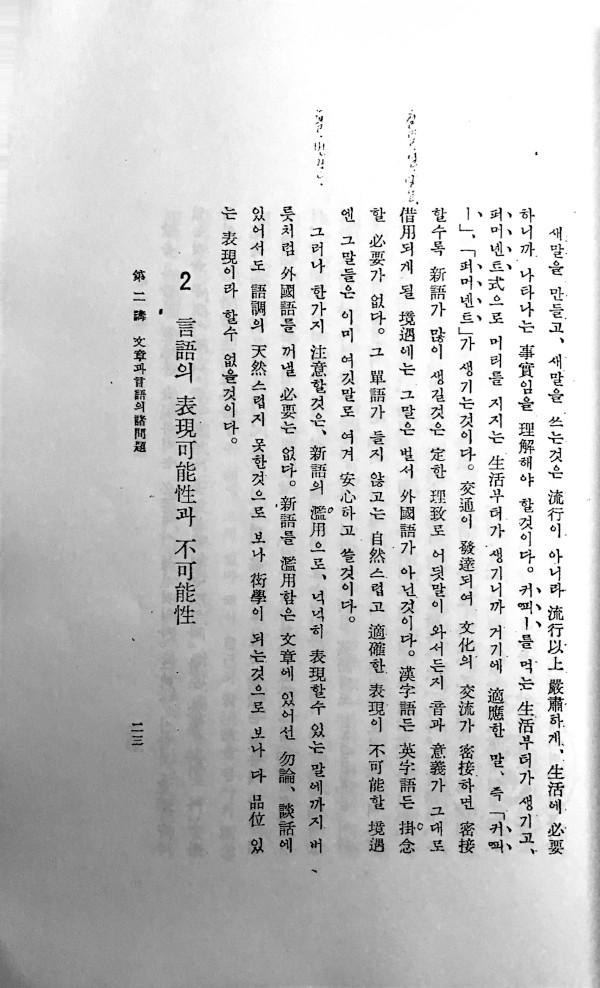
\includegraphics[width=9cm]{munjangganghwa}
\caption{이태준의 \ccnm{문장강화}의 한 페이지}\label{fig:mun}
\end{figure}

%\printindex

\end{document}